\documentclass{jot}

\usepackage[utf8]{inputenc}
\usepackage[T1]{fontenc}
\usepackage[english]{babel}
\usepackage{booktabs}
\usepackage{graphicx}
\graphicspath{{./figures/}}

\title{Nano-FFI: a comptime-generated, branch-free foreign function interface between Python and Zig}
\runningtitle{Nano-FFI: a branch-free Python/Zig FFI}

\author[affiliation=ir, nowrap]
    {Felipe Carvajal Brown}
    {holds an M.Sc. in Numerical Simulation in Engineering (Universidad Polit\'ecnica de Madrid, Spain) and works as an independent researcher in Santiago, Chile. Contact him at \email{fcarvajalbrown@gmail.com}.}

\affiliation{ir}{Independent Researcher, Santiago, Chile}

\runningauthor{Carvajal Brown}

\jotdetails{
    volume=0,
    number=0,
    articleno=0,
    year=2026,
    doisuffix=jot.2026.0.0.a0
}

\begin{document}

\begin{abstract}
Calling native code from Python is routine. The general-purpose bridges that make it convenient, \texttt{ctypes} and \texttt{cffi}, inspect argument types at call time, and that per-call cost dominates once the callee is small and called often. Nano-FFI moves the type dispatch to compile time instead. Given a Zig function and a declarative signature, its \texttt{makeTrampoline} runs Zig's \texttt{comptime} engine to generate a specialised wrapper whose argument unpacking compiles to straight-line code, with no runtime type inspection and no branch in the hot path. The bridge marshals 11 argument kinds, among them UTF-8 strings, raw bytes, zero-copy writable buffers, and multi-value tuple returns; Zig error unions map onto Python exceptions. On the reference platform a scalar call costs about 94~ns, roughly 3.5 times less than a minimal \texttt{ctypes} call. 42 end-to-end tests and the Zig unit suite cover the surface. Nano-FFI is released under the MIT license with a frozen 1.0 API.
\end{abstract}

\keywords{foreign function interface; Python; Zig; comptime; native extension; software}

\section{Introduction}

Python's reach into native code rests on a few well-worn tools. \texttt{ctypes} and \texttt{cffi} are popular because they need no compiler at the call site: the caller describes a function's argument and return types, and the library marshals values accordingly at run time. That flexibility has a price. Every call walks a description of the signature, dispatches on each argument's type, and boxes or unboxes values through general-purpose paths. When the native function does real work, the overhead vanishes into the noise. When it is a handful of instructions in a tight loop, the marshalling is most of the cost.

Compiled bridges avoid that by specialising ahead of time. Cython~\cite{cython} compiles annotated Python to C; pybind11 and PyO3 generate C++ or Rust glue whose type handling is fixed at build time. They are powerful, general, and correspondingly large. Nano-FFI aims lower. Its one idea is that the wrapper for each function should be generated, fully typed, at compile time, in a language whose compile-time execution model makes that natural.

That language is Zig~\cite{zig}. Zig's \texttt{comptime} runs ordinary code during compilation, over ordinary values, including a function and a description of its signature. Nano-FFI uses this directly. The argument-unpacking loop is a \texttt{comptime} \texttt{inline for} over the signature, so the compiler emits explicit typed assignments rather than a runtime loop with per-element type tests. What Python calls into, then, is a dispatch path with no branch left to resolve.

\section{Background}

A CPython extension module is a shared library that exposes an initialisation symbol and returns a module object populated with \texttt{PyMethodDef} entries. Inside those methods, values cross the boundary as \texttt{PyObject} pointers and convert to and from C types through the CPython C-API~\cite{capi}. \texttt{ctypes}~\cite{ctypes} and \texttt{cffi}~\cite{cffi} wrap that machinery behind a runtime type description, and the description is consulted on every call.

Specialising removes that step. If the exact types are known when the wrapper is built, the conversions can be emitted as fixed code. Cython, pybind11 and PyO3 all do this, from different source languages. Nano-FFI's contribution is not to compete with them on breadth but to show how small and how fast the bridge becomes when the wrapper generator is itself a compile-time program written in Zig's \texttt{comptime}.

\section{Design and implementation}

Nano-FFI holds one strict boundary. Exactly one source file, \texttt{python\_ext.zig}, includes \texttt{<Python.h>}; every other module is pure Zig over C-ABI-compatible types. That isolation keeps the CPython dependency in one place and lets the core (the trampoline generator and the registry) be unit-tested without a Python interpreter running at all.

\paragraph{Comptime trampolines.}
The core is \texttt{makeTrampoline(func, signature)}. It returns a wrapper of fixed C-ABI shape, \texttt{fn (args: [*]const RawArg) callconv(.c) RawRet}, that Python calls in place of \texttt{func}. The wrapper unpacks each argument at a comptime-known offset:

\begin{verbatim}
inline for (signature.args, 0..) |desc, i| {
    typed_args[i] = unpack(desc.typ, args[i]);
}
result = @call(.auto, func, typed_args);
\end{verbatim}

\noindent Because the loop is \texttt{inline} and the types are comptime, the compiler produces one typed assignment per argument, not a loop with runtime type checks. The return is handled the same way: \texttt{pack} picks the return conversion at compile time.

\paragraph{C-ABI marshalling.}
Values cross the internal boundary as an \texttt{extern struct} \texttt{RawArg \{tag, val\}}, where \texttt{val} is an \texttt{extern union} of the supported scalar representations plus a \texttt{RawSlice \{ptr, len\}} for variable-length data. Tagged unions are not C-ABI stable, so Nano-FFI carries an explicit tag alongside a C-compatible union instead. The return type \texttt{RawRet} holds the same union, an optional error pointer, and a small multi-return count.

\paragraph{Registry.}
A \texttt{StringHashMap} maps a name to a function pointer and its \texttt{Signature}. The dispatcher looks the entry up, checks arity, unpacks the Python tuple into a \texttt{RawArg} array, invokes the trampoline through the stored pointer, and converts the result back to a \texttt{PyObject}. The signature travels with the pointer, which is what later lets the module describe itself.

\section{Type system and safety}

Nano-FFI marshals 11 argument kinds: \texttt{i64}, \texttt{i32}, \texttt{u64}, \texttt{u32}, \texttt{u8}, \texttt{f64}, \texttt{f32}, \texttt{bool}, \texttt{str}, \texttt{bytes}, \texttt{buffer}. Three choices keep the boundary safe, not just fast.

Start with integer narrowing. A Python integer that will not fit the target width raises \texttt{ValueError} rather than truncating in silence. Unsigned targets reject negatives, and \texttt{u64} uses the full unsigned range.

Errors matter just as much. A wrapped Zig function may return an error union \texttt{E!T}. The trampoline unwraps it at compile time, so non-fallible functions keep the branch-free path, and on error it carries the Zig \texttt{@errorName} back. The Python layer raises that as a \texttt{RuntimeError} whose message is the error name.

The third choice is about memory. A \texttt{buffer} argument is a writable Python buffer, a \texttt{bytearray}, a writable \texttt{memoryview}, or a NumPy array, handed to Zig as a mutable \texttt{[]u8} that points straight at Python's own storage. Nothing is copied. The buffer is acquired with \texttt{PyObject\_GetBuffer(PyBUF\_WRITABLE)} and released after the call; a read-only object is rejected with \texttt{BufferError}.

The module is self-describing. \texttt{list\_functions()} returns the registered names (14 built-in examples ship with the module), and \texttt{signature(name)} returns the argument names and types and the return type, with a list of types when the return is multi-value. PEP 561 stubs and a \texttt{py.typed} marker ship in the wheel.

\section{Verification}

Correctness is checked at two levels. The pure-Zig core (trampoline generation, registry, allocator boundary) runs under Zig unit tests that need no Python interpreter, through a dedicated test root that leaves the \texttt{<Python.h>} module out. The full boundary is covered by 42 end-to-end tests in CPython that call every built-in example across every type, and that includes the overflow, wrong-arity, empty-input, read-only-buffer, and divide-by-zero error paths. Both suites pass on the reference platform.

\section{Performance}

I measure the wall-clock cost of a single call, averaged over 100\,000 iterations after a warm-up, and report the median of 5 repeats to damp scheduler noise. The baseline is a minimal \texttt{ctypes} call into a trivial libc function (\texttt{abs}/\texttt{fabs}). That is a reference for dispatch overhead, not a like-for-like of the same computation. Every measurement uses a \texttt{ReleaseFast} build.

On CPython 3.14 (Windows x64) the scalar \texttt{add(i64, i64)} call costs about 94~ns. A float multiply costs about 105~ns, a string-length call about 86~ns, a two-value \texttt{divmod} return about 121~ns, and a zero-copy buffer fill about 120~ns. The minimal \texttt{ctypes} baseline is about 334~ns, so a scalar Nano-FFI call carries roughly 3.5 times less overhead. The variable-length and multi-value paths cost more than the scalar path, as one would expect, and both stay well under the general-purpose baseline.

\begin{table}[ht]
\centering
\begin{tabular}{lr}
\toprule
Call kind & Overhead (ns/call) \\
\midrule
scalar (\texttt{add} i64) & 94 \\
float (\texttt{mul} f64) & 105 \\
string (\texttt{strlen}) & 86 \\
multi-return (\texttt{divmod}) & 121 \\
zero-copy buffer (\texttt{fill}) & 120 \\
\texttt{ctypes} baseline & 334 \\
\bottomrule
\end{tabular}
\caption{Median per-call overhead by kind, versus a minimal \texttt{ctypes} baseline.}
\label{tab:perf}
\end{table}

\begin{figure}[ht]
\centering
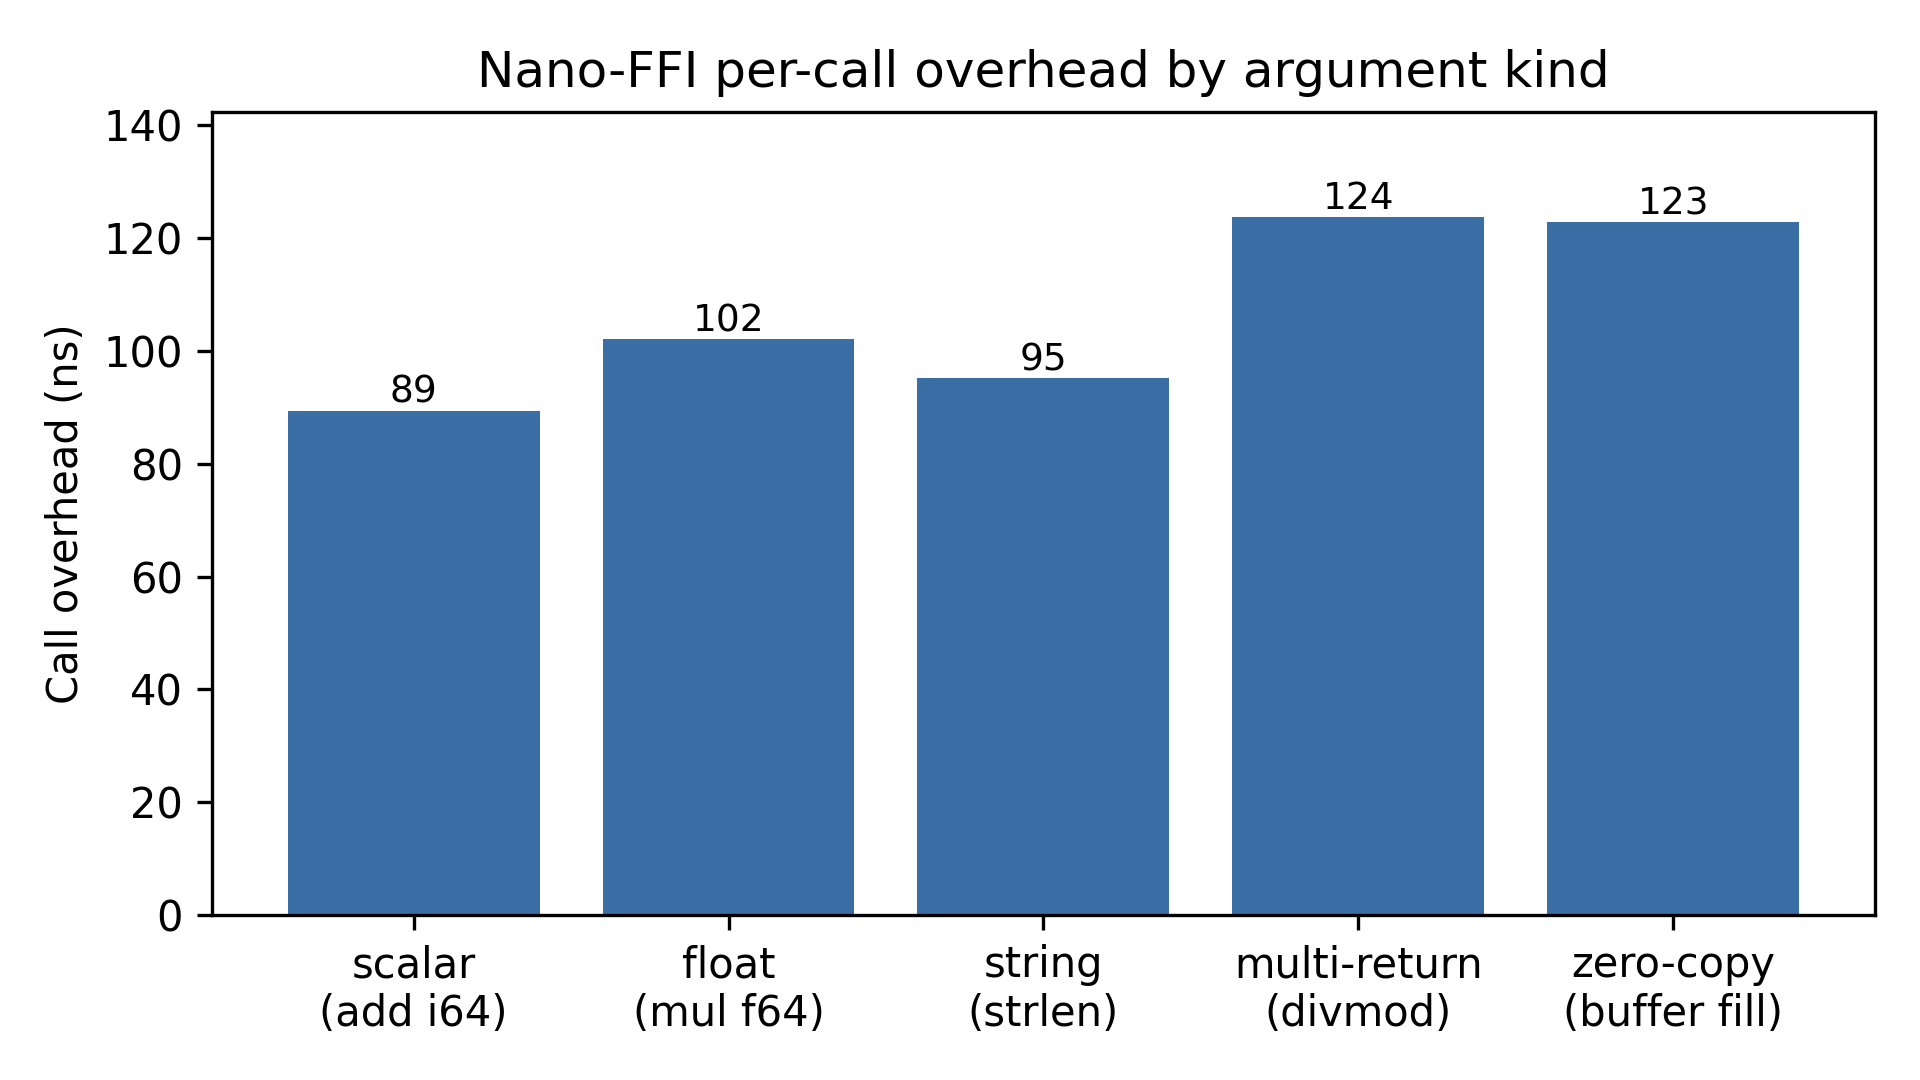
\includegraphics[width=0.82\textwidth]{fig_overhead.png}
\caption{Per-call overhead by argument kind.}
\label{fig:overhead}
\end{figure}

\begin{figure}[ht]
\centering
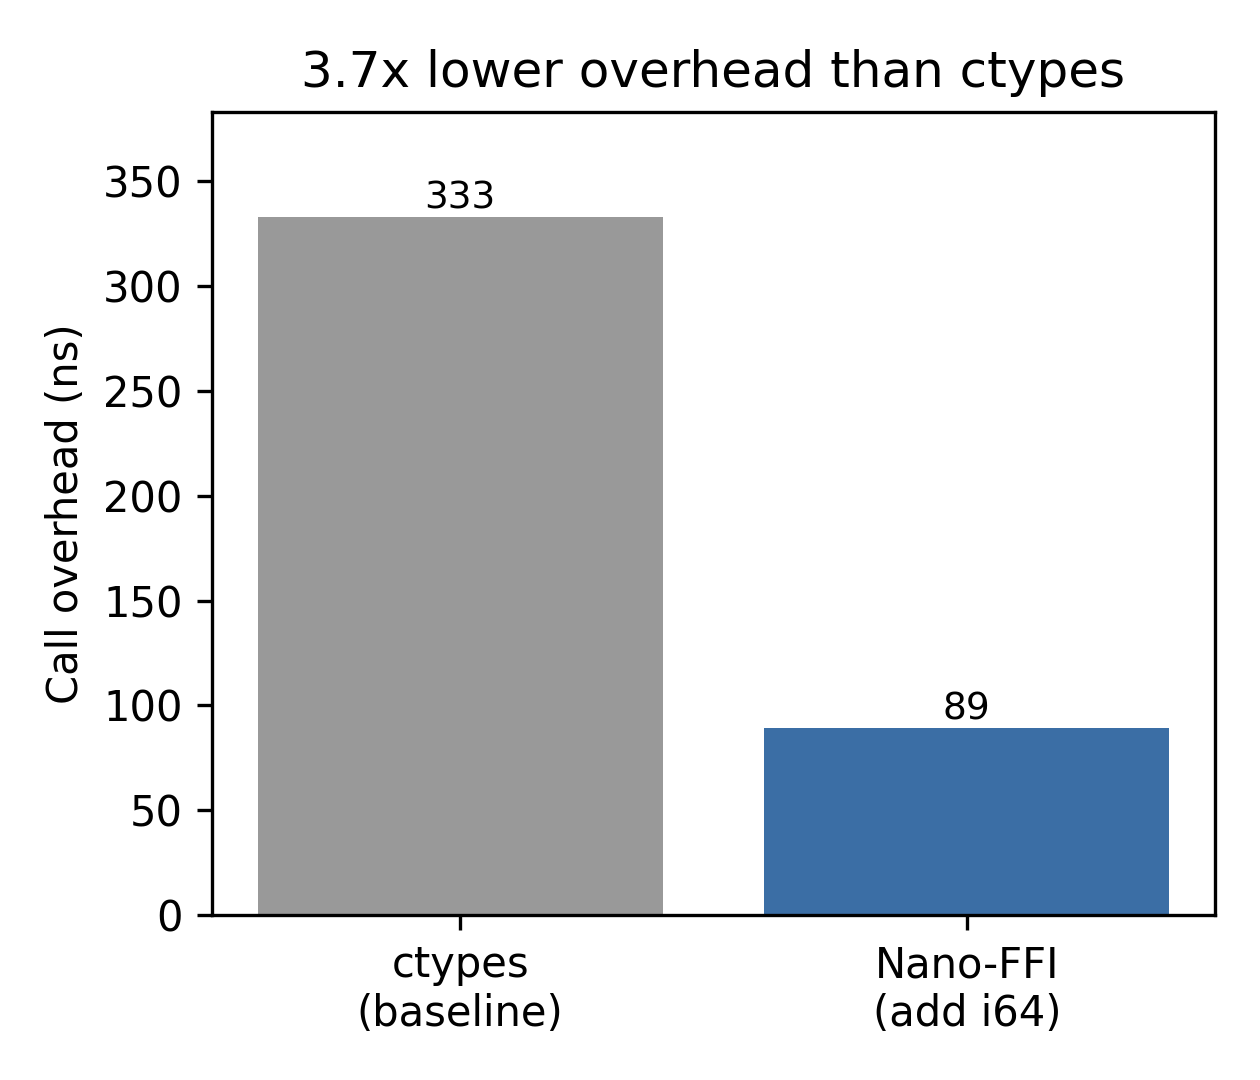
\includegraphics[width=0.5\textwidth]{fig_vs_ctypes.png}
\caption{Scalar call overhead versus the \texttt{ctypes} baseline.}
\label{fig:vsctypes}
\end{figure}

\section{Discussion and limitations}

The benchmark measures dispatch overhead, not application throughput. For native functions that do substantial work the bridge cost is irrelevant, and Nano-FFI's advantage is confined to the small-callee, high-frequency regime it is built for. The comparison function is not the baseline's callee, so the ratio is best read as the cost of crossing the boundary, not a speedup of identical work. Two structural limits remain. The bridge caps arguments and return values at eight each, and a Zig-returned slice must be valid at the moment of return, whether static data or a view into the arguments; returning owned heap buffers is future work. The reported numbers are also single-platform. The build matrix covers Linux, Windows and macOS, but the quoted overhead is the Windows reference run.

\section{Availability}

Nano-FFI is open source under the MIT license. The 1.0 release freezes the public API (\texttt{call}, \texttt{version}, \texttt{list\_functions}, \texttt{signature}), the supported type names, and the exception mapping, and follows semantic versioning from there. Source, tests, the benchmark harness, and this manuscript's build scripts live in the repository. The extension builds with Zig 0.15.2 against CPython 3.10 or newer.

\backmatter

\begin{thebibliography}{9}
\bibitem{cython} S. Behnel, R. Bradshaw, C. Citro, L. Dalcin, D. S. Seljebotn, and K. Smith, ``Cython: The Best of Both Worlds,'' \emph{Computing in Science \& Engineering}, vol. 13, no. 2, pp. 31--39, 2011. \url{https://doi.org/10.1109/MCSE.2010.118}
\bibitem{zig} The Zig Programming Language. \url{https://ziglang.org}
\bibitem{capi} Python/C API Reference Manual. \url{https://docs.python.org/3/c-api/}
\bibitem{ctypes} ctypes --- A foreign function library for Python. \url{https://docs.python.org/3/library/ctypes.html}
\bibitem{cffi} CFFI --- C Foreign Function Interface for Python. \url{https://cffi.readthedocs.io}
\end{thebibliography}

\abouttheauthors

\end{document}
